\documentclass[aspectratio=169,11pt]{beamer}

\usetheme{Madrid}
\usecolortheme{default}
\usefonttheme{professionalfonts}
\setbeamertemplate{navigation symbols}{}
\setbeamertemplate{footline}[frame number]
\setbeamertemplate{caption}[numbered]

\usepackage{amsmath}
\usepackage{amssymb}
\usepackage{booktabs}
\usepackage{graphicx}
\usepackage{xurl}

\graphicspath{{../figures/}}

\title[FFT Diffraction]{FFT-Based Fraunhofer Diffraction}
\subtitle{Algorithms, Sampling Design, and Error Analysis}
\author[Ruijie Li]{24300720157 Ruijie Li}
\institute{}
\date{\today}

\DeclareMathOperator{\sinc}{sinc}

\begin{document}

\begin{frame}
    \titlepage
\end{frame}

\begin{frame}{Main Question}
    Fraunhofer diffraction is formally a Fourier transform, so the FFT is the natural numerical tool.
    The central issue is that the FFT also imposes a sampling grid.

    \vspace{0.4cm}
    \begin{block}{Goal}
        Build a reliable FFT diffraction solver by connecting physical approximations, grid design rules,
        error analysis, and numerical experiments.
    \end{block}

    \vspace{0.2cm}
    The final physical target is to recover the Rayleigh resolution scale
    \(1.22\lambda/D\) from the computed Airy pattern.
\end{frame}

\begin{frame}{Talk Structure}
    \begin{enumerate}
        \item Physical model: Helmholtz \(\to\) angular spectrum \(\to\) Fraunhofer.
        \item Numerical discretization: continuous Fourier integral \(\to\) DFT \(\to\) screen grid.
        \item Algorithms: FFT propagator, Simpson reference, ASM reference, Rayleigh recovery.
        \item Error analysis: E1 aliasing, E2 screen resolution, E3 model error.
        \item Experiments: analytical validation, convergence, grid rules, breakdown, efficiency, Rayleigh.
    \end{enumerate}
\end{frame}

\section{Theory}

\begin{frame}{Fouier Transform Convention}
    We use the transform pair
    \[
        \hat{f}(\xi,\eta)
        =
        \int_{\mathbb{R}^2}
        f(x,y)\mathrm{e}^{-2\pi\mathrm{i}(x\xi+y\eta)}
        \,\mathrm{d}x\,\mathrm{d}y,
    \]
    \[
        f(x,y)
        =
        \int_{\mathbb{R}^2}
        \hat{f}(\xi,\eta)\mathrm{e}^{2\pi\mathrm{i}(x\xi+y\eta)}
        \,\mathrm{d}\xi\,\mathrm{d}\eta.
    \]

    \vspace{0.15cm}
    With this convention, partial derivatives become multiplication in the frequency domain:
    \[
        \widehat{\frac{\partial f}{\partial x}}(\xi,\eta)
        =
        2\pi\mathrm{i}\xi\hat{f}(\xi,\eta),\qquad
        \widehat{\frac{\partial f}{\partial y}}(\xi,\eta)
        =
        2\pi\mathrm{i}\eta\hat{f}(\xi,\eta).
    \]
    Hence
    \[
        \widehat{\frac{\partial^2 f}{\partial x^2}}(\xi,\eta)
        =
        -4\pi^2\xi^2\hat{f}(\xi,\eta),\qquad
        \widehat{\frac{\partial^2 f}{\partial y^2}}(\xi,\eta)
        =
        -4\pi^2\eta^2\hat{f}(\xi,\eta).
    \]
\end{frame}

\begin{frame}{Scalar Wave Model}
    A monochromatic scalar field is written as
    \[
        U(x,y,z,t)=U(x,y,z)\mathrm{e}^{-\mathrm{i}\omega t}.
    \]
    In a homogeneous source-free region, the spatial part satisfies the Helmholtz equation
    \[
        \Delta U+k^2U=0,\qquad k=\frac{2\pi}{\lambda}.
    \]

    \vspace{0.2cm}
    The aperture field \(A(x,y)=U(x,y,0)\) is propagated from the aperture plane to a screen at distance
    \(z\).
\end{frame}

\begin{frame}{Angular Spectrum Representation}
    Taking the two-dimensional Fourier transform in \(x,y\) diagonalizes the transverse derivatives.
    For each spatial frequency \((f_x,f_y)\), the Helmholtz equation becomes
    \[
        \frac{\partial^2\hat{U}}{\partial z^2}
        +k_z(f_x,f_y)^2\hat{U}=0,
        \qquad
        k_z^2=4\pi^2\left(\frac{1}{\lambda^2}-f_x^2-f_y^2\right).
    \]

    The transfer function is therefore
    \[
        H(f_x,f_y,z)=
        \begin{cases}
            \mathrm{e}^{\mathrm{i}k_z(f_x,f_y)z}, & f_x^2+f_y^2<\lambda^{-2},\\
            \mathrm{e}^{-\sqrt{-k_z(f_x,f_y)^2}\,z}, & f_x^2+f_y^2>\lambda^{-2}.
        \end{cases}
    \]

    Hence the angular-spectrum solution is \(U(x,y,z)=\mathcal{F}^{-1}\{\hat{A}(f_x,f_y)H(f_x,f_y,z)\}\).
\end{frame}

\begin{frame}{Approximation Ladder}
    The physical models form a hierarchy:

    \vspace{0.2cm}
    \begin{center}
    \begin{tabular}{lll}
        \toprule
        Model & Valid regime & Numerical role \\
        \midrule
        Angular spectrum & general propagation & reference \\
        Fresnel & paraxial propagation & near/far transition \\
        Fraunhofer & far field, small Fresnel number & main FFT solver \\
        \bottomrule
    \end{tabular}
    \end{center}

    \vspace{0.25cm}
    The Fresnel number \(F=a^2/(\lambda z)\) is the key dimensionless quantity controlling the
    Fraunhofer model error.
\end{frame}

\begin{frame}{Fresnel Approximation}
    For paraxial waves, \(f_x^2+f_y^2\ll \lambda^{-2}\), so
    \[
        \sqrt{\lambda^{-2}-(f_x^2+f_y^2)}
        \approx
        \frac{1}{\lambda}-\frac{\lambda}{2}(f_x^2+f_y^2).
    \]
    This gives the Fresnel transfer function
    \[
        H_F(f_x,f_y;z)
        =
        \mathrm{e}^{\mathrm{i}kz}
        \mathrm{e}^{-\mathrm{i}\pi\lambda z(f_x^2+f_y^2)}.
    \]

    \vspace{0.15cm}
    Fraunhofer is obtained from Fresnel by further neglecting the aperture-plane quadratic phase in the
    far-field regime.
\end{frame}

\begin{frame}{Fraunhofer Formula}
    In the far field, the screen field is proportional to the Fourier transform of the aperture:
    \[
        U(X,Y;z)
        \propto
        \hat{A}\!\left(\frac{X}{\lambda z},\frac{Y}{\lambda z}\right).
    \]

    \vspace{0.2cm}
    Thus the frequency-screen correspondence is
    \[
        X=\lambda z f_x,\qquad Y=\lambda z f_y.
    \]

    \vspace{0.2cm}
    This simple relation is what converts the FFT frequency grid into a physical screen grid.
\end{frame}

\section{Discretization}

\begin{frame}{From the Aperture Grid to FFT Frequencies}
    Use a square computational window \(W_L=[-L/2,L/2)^2\), with \(L=N\Delta x\). The centered aperture
    grid is
    \[
        x_m=\left(m-\frac{N}{2}\right)\Delta x,\qquad
        y_n=\left(n-\frac{N}{2}\right)\Delta x,
        \qquad 0\le m,n\le N-1.
    \]

    \vspace{0.15cm}
    The Fourier transform is approximated by the rectangle rule:
    \[
        \hat{A}(f_x,f_y)
        \approx
        \Delta x^2
        \sum_{m=0}^{N-1}\sum_{n=0}^{N-1}
        A_{m,n}
        \mathrm{e}^{-2\pi\mathrm{i}(x_mf_x+y_nf_y)}.
    \]

    \vspace{0.15cm}
    Matching this phase with the DFT kernel forces \(f_x\Delta x=p/N\) and
    \(f_y\Delta x=q/N\). In centered order,
    \[
        f_p=\frac{p-N/2}{N\Delta x},\qquad
        f_q=\frac{q-N/2}{N\Delta x}.
    \]
\end{frame}

\begin{frame}{Centered FFT Convention}
    The centered physical grid introduces a phase convention, handled in code by shifts:
    \[
    \hat{A}(f_p,f_q)
    \approx
    \Delta x^2
    \operatorname{fftshift}\!\left(
        \operatorname{fft2}\!\left(\operatorname{ifftshift}(A)\right)
    \right)_{p,q}.
    \]

    \vspace{0.2cm}
    \begin{itemize}
        \item \(\operatorname{ifftshift}\): move the physical center to the DFT origin before applying FFT.
        \item \(\operatorname{fftshift}\): put zero frequency back at the center for plotting.
        \item The FFT is still the rectangle-rule approximation of the continuous Fourier transform.
    \end{itemize}
\end{frame}

\begin{frame}{Screen Coordinates Induced by the FFT}
    Fraunhofer requires \(X/(\lambda z)=f_x\), so
    \[
        X_p=\lambda z f_p,\qquad Y_q=\lambda z f_q.
    \]

    \vspace{0.15cm}
    The three key grid relations are
    \[
        \Delta X=\frac{\lambda z}{L},\qquad
        X_{\max}\approx \frac{\lambda z}{2\Delta x},\qquad
        N=\frac{L}{\Delta x}.
    \]

    \vspace{0.2cm}
    \begin{block}{Interpretation}
        \(L\) controls screen resolution; \(\Delta x\) controls observable screen range.
    \end{block}
\end{frame}

\begin{frame}{Grid Design Rules}
    For a target screen range \(X_{\max}^{\mathrm{tgt}}\), target screen spacing
    \(\Delta X^{\mathrm{tgt}}\), and aperture scale \(a\), use
    \[
        \Delta x\leq \frac{\lambda z}{2X_{\max}^{\mathrm{tgt}}},
        \qquad
        L\geq \frac{\lambda z}{\Delta X^{\mathrm{tgt}}}.
    \]
    \[
        L\geq 2a,\qquad
        \Delta x\leq \frac{a}{k_{\mathrm{edge}}}.
    \]

    \vspace{0.15cm}
    A practical choice is
    \[
        \Delta x=\min\!\left\{\frac{\lambda z}{2X_{\max}^{\mathrm{tgt}}},
        \frac{a}{k_{\mathrm{edge}}}\right\},\qquad
        L_{\min}=\max\!\left\{2a,\frac{\lambda z}{\Delta X^{\mathrm{tgt}}}\right\}.
    \]
    Then choose \(N\) so that \(N\Delta x\geq L_{\min}\), usually rounded to a convenient FFT size.
\end{frame}

\begin{frame}{What Increasing \(N\) Really Means}
    \begin{columns}[T,onlytextwidth]
        \column{0.48\textwidth}
        \begin{block}{Fixed \(\Delta x\)}
            \(L=N\Delta x\) increases.

            \[
                \Delta X=\frac{\lambda z}{L}\downarrow,\qquad
                X_{\max}\ \text{unchanged}.
            \]
        \end{block}

        \column{0.48\textwidth}
        \begin{block}{Fixed \(L\)}
            \(\Delta x=L/N\) decreases.

            \vspace{0.1cm}
            This refines aperture sampling:
            \[
                X_{\max}\approx\frac{\lambda z}{2\Delta x}\uparrow,\qquad
                \Delta X\ \text{unchanged}.
            \]
        \end{block}
    \end{columns}

    \vspace{0.15cm}
    Thus aliasing is controlled mainly by \(\Delta x\), while screen resolution is controlled mainly by
    \(L\).
\end{frame}

\section{Algorithms and Error}

\begin{frame}{Algorithm Roles}
    \begin{center}
    \begin{tabular}{lll}
        \toprule
        Method & Cost & Purpose \\
        \midrule
        Fraunhofer FFT & \(O(N^2\log N)\) & main far-field solver \\
        Simpson quadrature & \(O(N^4)\) & direct integral check \\
        Angular spectrum & \(O(N^2\log N)\) & propagation reference \\
        Rayleigh recovery & post-processing & physical validation \\
        \bottomrule
    \end{tabular}
    \end{center}

    \vspace{0.2cm}
    The reference methods prevent the project from relying on a single implementation of the FFT formula.
\end{frame}

\begin{frame}{Fraunhofer FFT Propagator}
    Given a centered aperture array \(A\), the main computation is
    \[
        U^{\mathrm{Fh}}_{p,q}
        =
        \Delta x^2
        \operatorname{fftshift}\!\left(
            \operatorname{fft2}\!\left(\operatorname{ifftshift}(A)\right)
        \right)_{p,q}.
    \]

    \vspace{0.15cm}
    The screen coordinates are
    \[
        X_p=\lambda z\frac{p-N/2}{N\Delta x},\qquad
        Y_q=\lambda z\frac{q-N/2}{N\Delta x}.
    \]

    \vspace{0.15cm}
    Intensities are compared after peak normalization, so the global factor \(1/(\lambda^2 z^2)\) is
    omitted in most experiments.
\end{frame}

\begin{frame}{Reference Computations and Rayleigh Recovery}
    \begin{itemize}
        \item \textbf{Simpson quadrature:} evaluates the Fraunhofer integral directly at prescribed screen
              points. On an \(N\times N\) aperture and an \(N\times N\) screen, the cost is \(O(N^4)\).
        \item \textbf{ASM:} computes
              \(U(\cdot,\cdot,z)=\mathcal{F}^{-1}\{\mathcal{F}\{A\}H\}\), so it is used as a propagation
              reference when Fraunhofer may fail.
        \item \textbf{Rayleigh recovery:} compute the Airy pattern, extract the central cut, locate the
              first dark ring, and return
              \[
                  c_{\mathrm{num}}=\frac{r_1D}{\lambda z}.
              \]
    \end{itemize}

    \vspace{0.1cm}
    The expected circular-aperture value is \(c=1.2196699\ldots\).
\end{frame}

\begin{frame}{Error Metrics}
    Intensities are peak-normalized before comparing shapes:
    \[
        \bar{I}=\frac{I}{\max I}.
    \]

    \vspace{0.15cm}
    The main relative error is
    \[
        \mathrm{Err}_2(I_{\mathrm{num}},I_{\mathrm{ref}})
        =
        \frac{\|\bar{I}_{\mathrm{num}}-\bar{I}_{\mathrm{ref}}\|_2}
        {\|\bar{I}_{\mathrm{ref}}\|_2}.
    \]

    \vspace{0.15cm}
    We also compare shape features such as FWHM, first-null location, and the Rayleigh constant when those
    are more physically meaningful.
\end{frame}

\begin{frame}{Error Decomposition}
    \begin{center}
    \begin{tabular}{cll}
        \toprule
        Symbol & Meaning & Controlled by \\
        \midrule
        E1 & aliasing error & \(\Delta x\), through \(X_{\max}\approx\lambda z/(2\Delta x)\) \\
        E2 & screen-resolution error & \(L\), through \(\Delta X=\lambda z/L\) \\
        E3 & Fraunhofer model error & \(F=a^2/(\lambda z)\) \\
        \bottomrule
    \end{tabular}
    \end{center}

    \vspace{0.2cm}
    \begin{itemize}
        \item E1 folds unresolved high-frequency content into the computed pattern.
        \item E2 under-samples fringes, nulls, or sidelobes on the screen.
        \item E3 comes from dropping the Fresnel quadratic phase; its largest omitted phase is
              \(\Delta\phi_{\max}=\pi F\).
    \end{itemize}
\end{frame}

\section{Experiments}

\begin{frame}{Experiment Design}
    \begin{center}
    \begin{tabular}{cll}
        \toprule
        Exp. & Purpose & Main mechanism \\
        \midrule
        1 & analytical validation & normalization and coordinates \\
        2 & convergence rates & smoothness of aperture \\
        3 & grid-design tightness & E1 and E2 \\
        4 & Fraunhofer breakdown & E3 and Fresnel number \\
        5 & efficiency comparison & FFT versus quadrature \\
        6 & Rayleigh recovery & physical resolution limit \\
        7 & complex apertures & qualitative Fourier optics \\
        \bottomrule
    \end{tabular}
    \end{center}
\end{frame}

\begin{frame}{Experiment 1: Analytical Validation}
    \begin{columns}[T,onlytextwidth]
        \column{0.54\textwidth}
        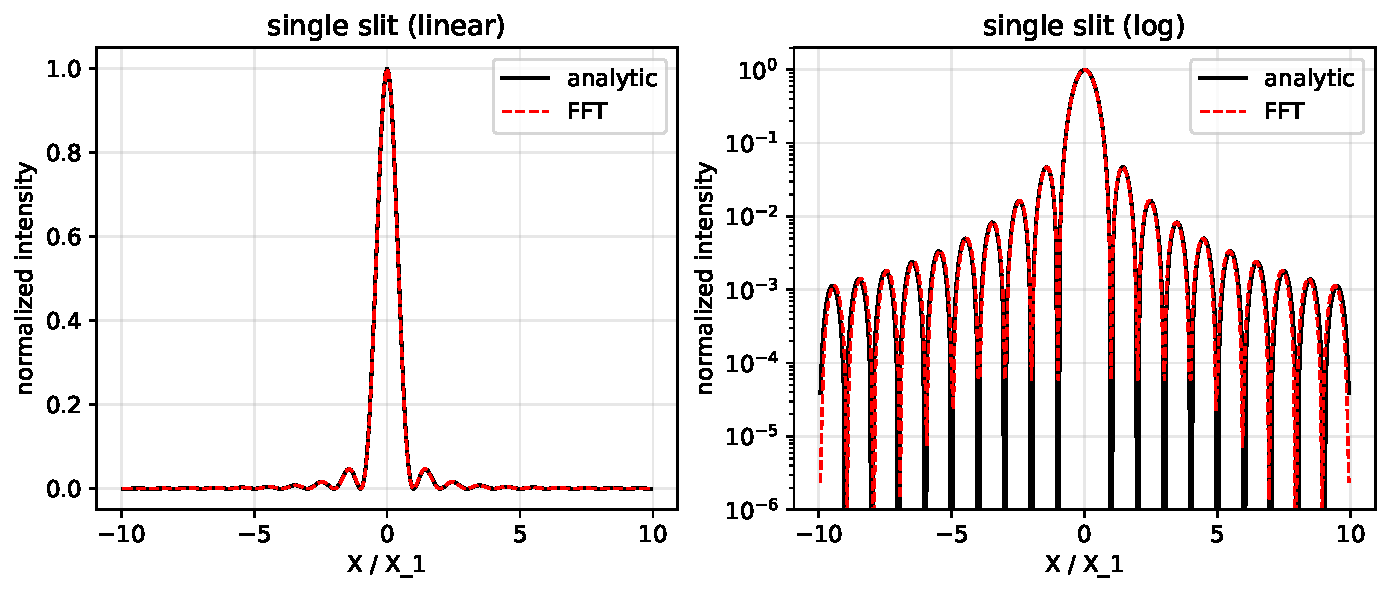
\includegraphics[width=\textwidth]{experiment1_single_slit.pdf}

        \vspace{0.1cm}
        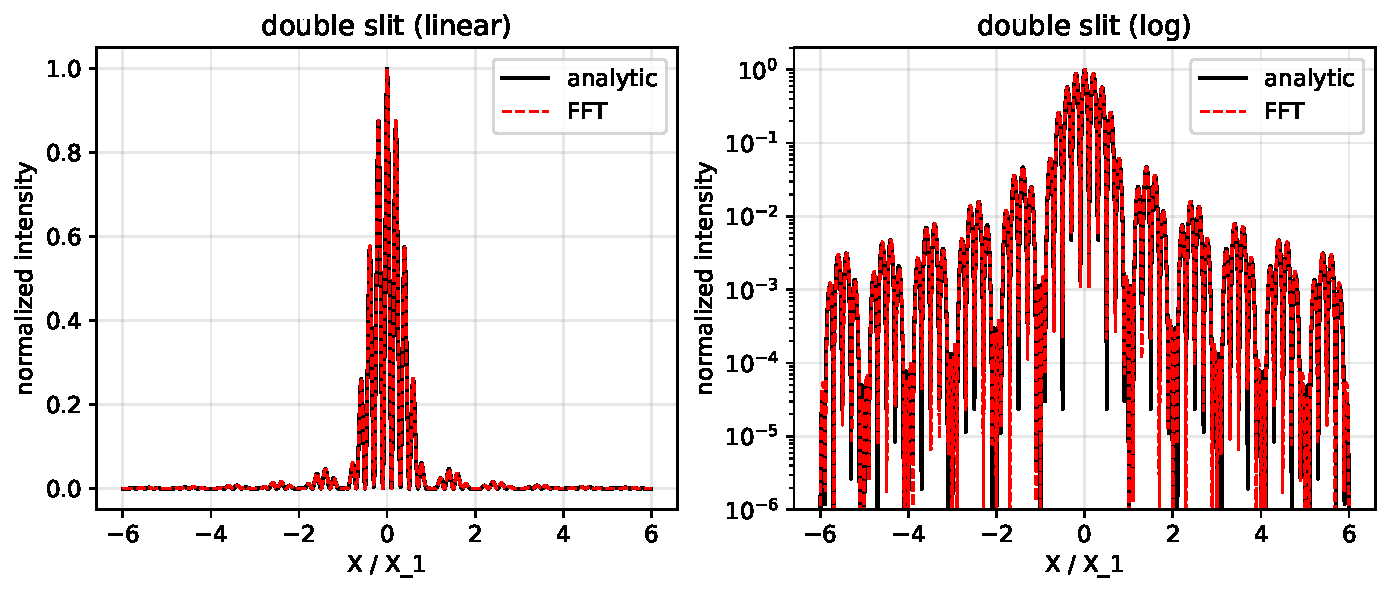
\includegraphics[width=\textwidth]{experiment1_double_slit.pdf}

        \column{0.42\textwidth}
        \small
        Closed-form tests:
        \begin{itemize}
            \item single slit: \(\sinc^2\)
            \item double slit: \(\sinc^2\cos^2\)
            \item rectangle: product of sinc terms
            \item circle: Airy pattern
        \end{itemize}

        \vspace{0.15cm}
        All relative errors are below \(1.5\%\). The circular aperture recovers the first Airy null with
        relative error \(1.74\times10^{-4}\).
    \end{columns}
\end{frame}

\begin{frame}{Experiment 1: Two-Dimensional Apertures}
    \begin{columns}[T,onlytextwidth]
        \column{0.50\textwidth}
        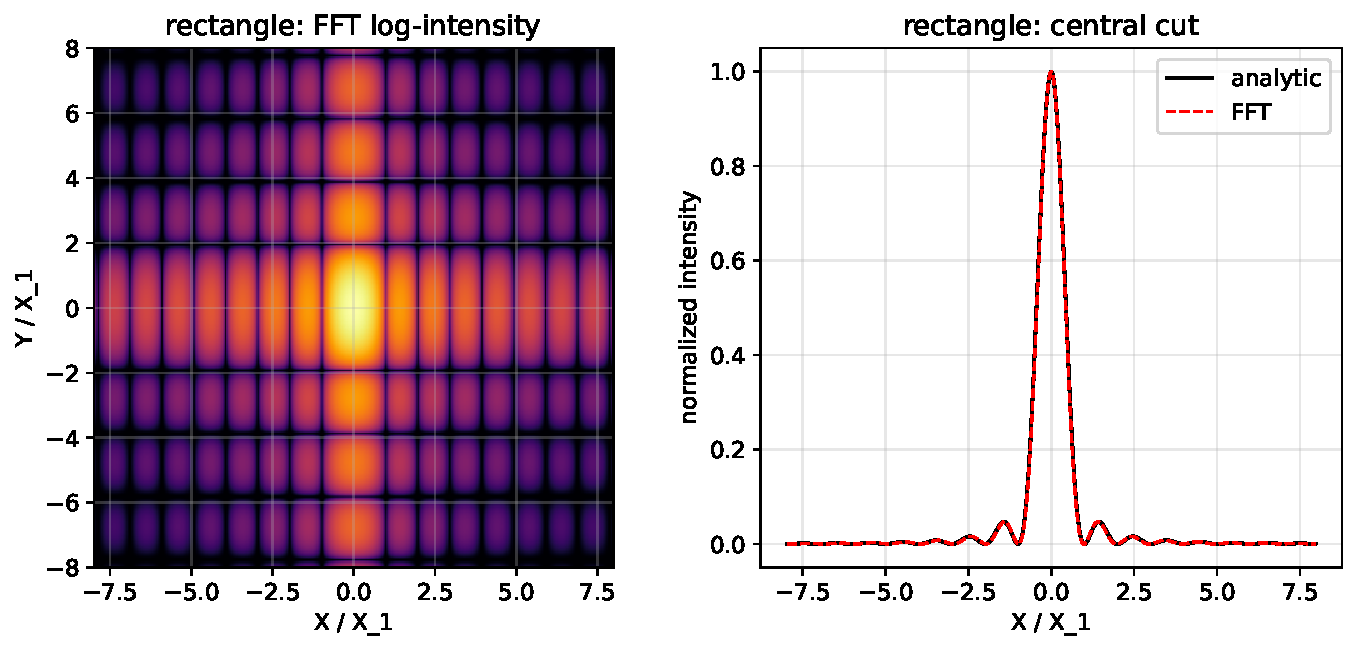
\includegraphics[width=\textwidth]{experiment1_rectangle.pdf}

        \column{0.50\textwidth}
        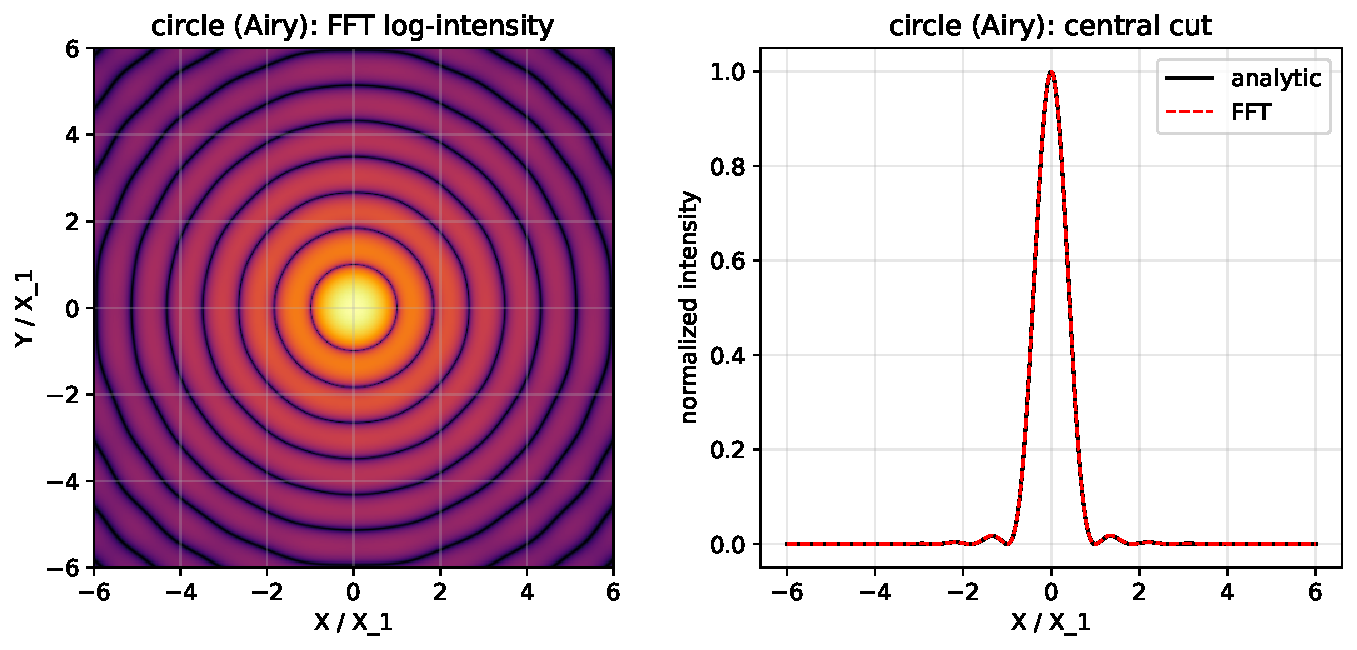
\includegraphics[width=\textwidth]{experiment1_circle.pdf}
    \end{columns}

    \vspace{0.1cm}
    \small
    The rectangular aperture validates the product sinc pattern. The circular aperture validates the Airy
    pattern and provides the basis for the Rayleigh recovery experiment.
\end{frame}

\begin{frame}{Experiment 2: Convergence Rates}
    \begin{columns}[T,onlytextwidth]
        \column{0.60\textwidth}
        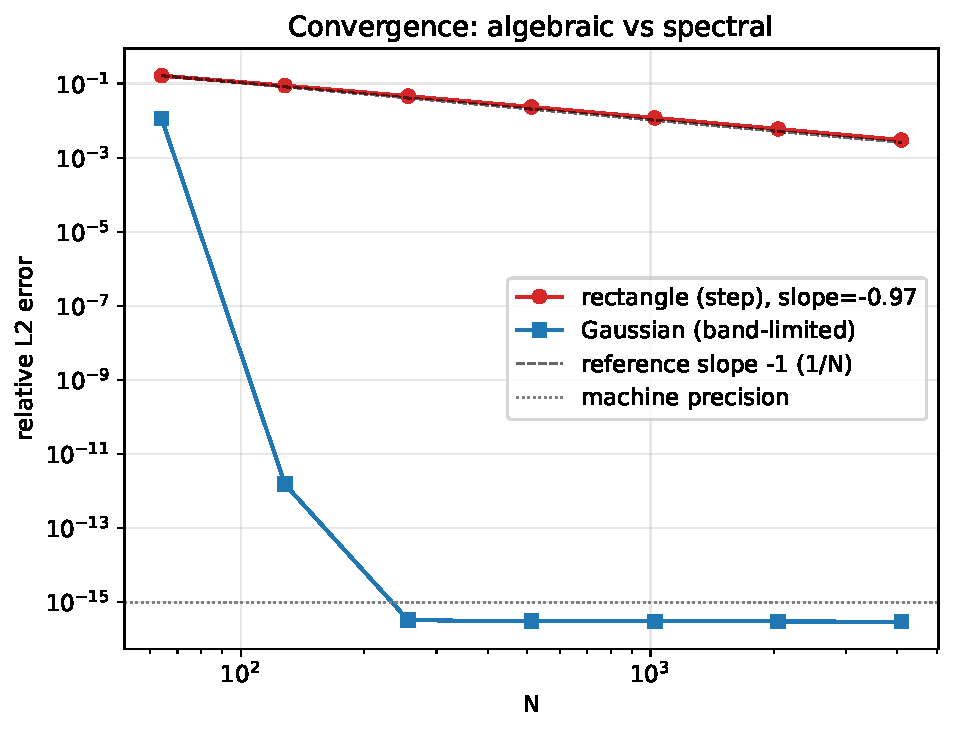
\includegraphics[width=\textwidth]{experiment2_convergence.pdf}

        \column{0.36\textwidth}
        \small
        The physical window is fixed and \(N\) is increased.

        \vspace{0.2cm}
        \begin{itemize}
            \item Square aperture: fitted slope \(-0.967\), close to \(O(1/N)\).
            \item Gaussian aperture: reaches machine precision by \(N=256\).
        \end{itemize}

        \vspace{0.1cm}
        Smoothness of the aperture controls spectral decay and convergence.
    \end{columns}
\end{frame}

\begin{frame}{Experiment 3: Grid Design Tightness}
    \begin{center}
        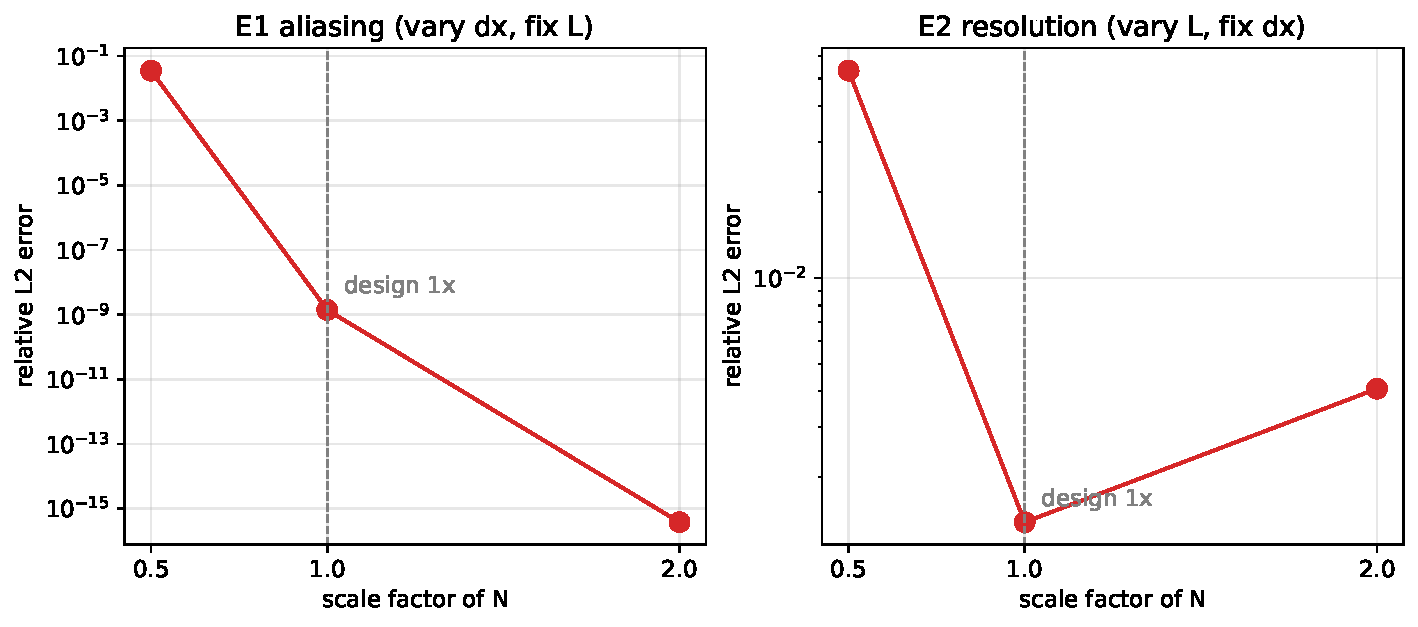
\includegraphics[width=0.49\textwidth,height=0.55\textheight,keepaspectratio]{experiment3_tightness.pdf}
        \hfill
        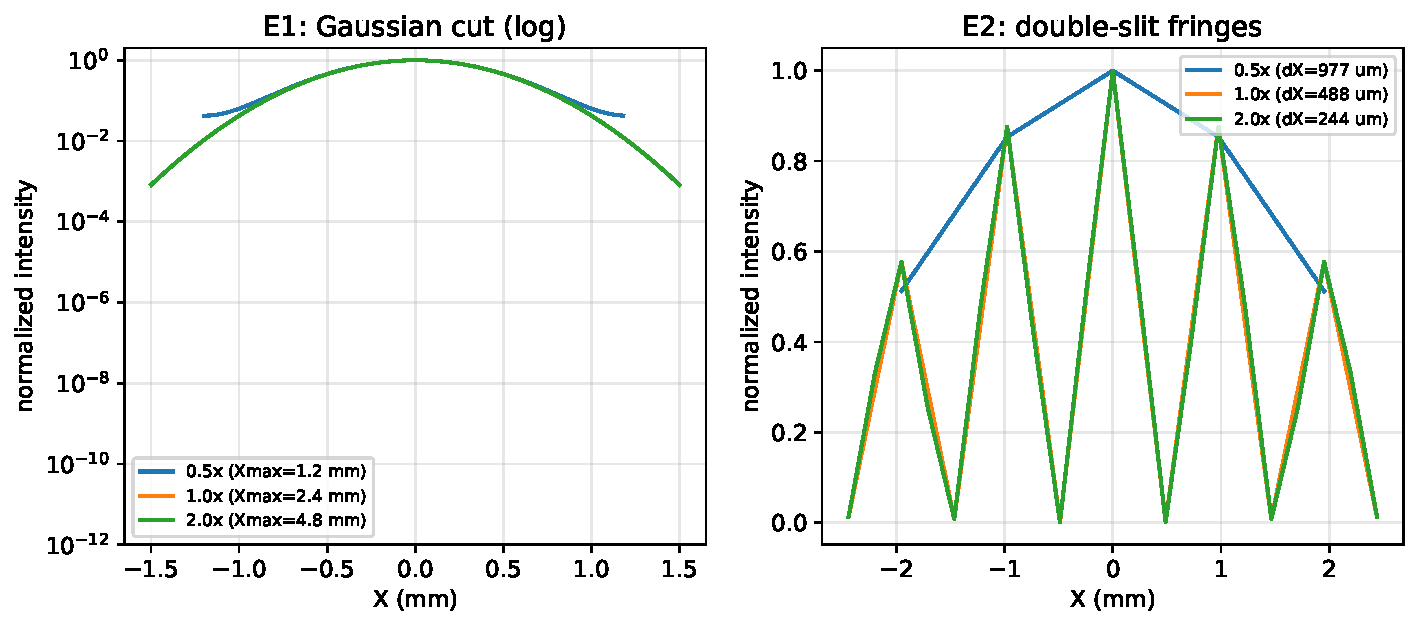
\includegraphics[width=0.49\textwidth,height=0.55\textheight,keepaspectratio]{experiment3_patterns.pdf}
    \end{center}

    \vspace{-0.15cm}
    \footnotesize
    \begin{center}
    \begin{tabular}{c|ccc}
        \toprule
        Scale & \(0.5\times\) & \(1\times\) design & \(2\times\) \\
        \midrule
        E1 aliasing & \(3.55\%\) & \(1.40\times10^{-9}\) & \(3.79\times10^{-16}\) \\
        E2 resolution & \(5.33\%\) & \(0.14\%\) & \(0.41\%\) \\
        \bottomrule
    \end{tabular}
    \end{center}

    \vspace{-0.10cm}
    \small
    Half-size grids fail visibly; the designed grid is already near the useful threshold.
\end{frame}

\begin{frame}{Experiment 4: Fraunhofer Breakdown}
    \begin{center}
        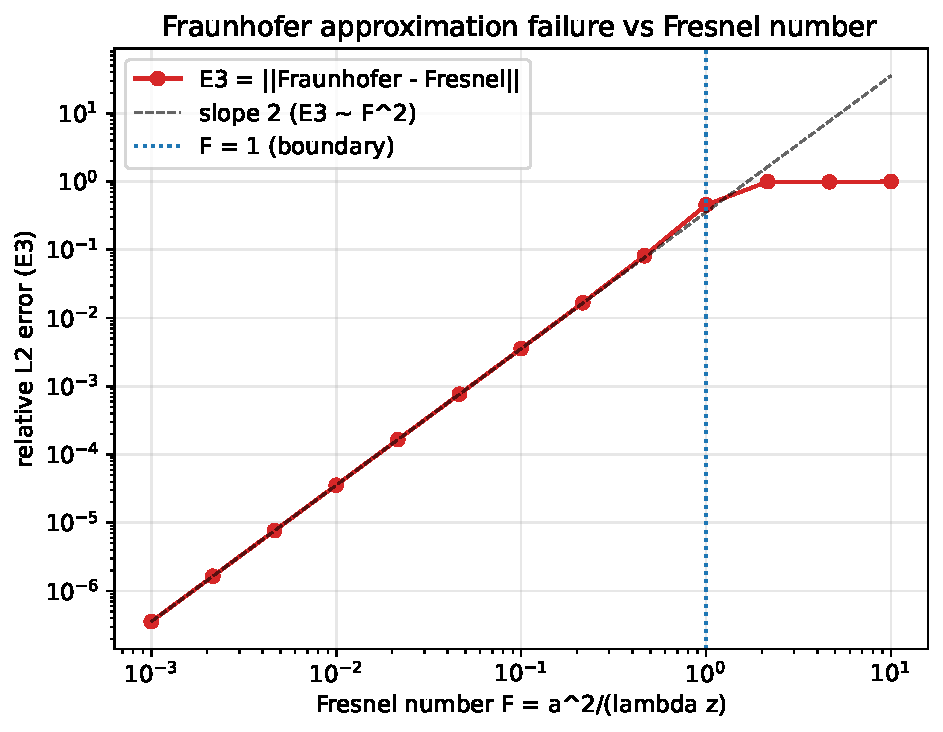
\includegraphics[width=0.49\textwidth,height=0.58\textheight,keepaspectratio]{experiment4_e3_vs_fresnel.pdf}
        \hfill
        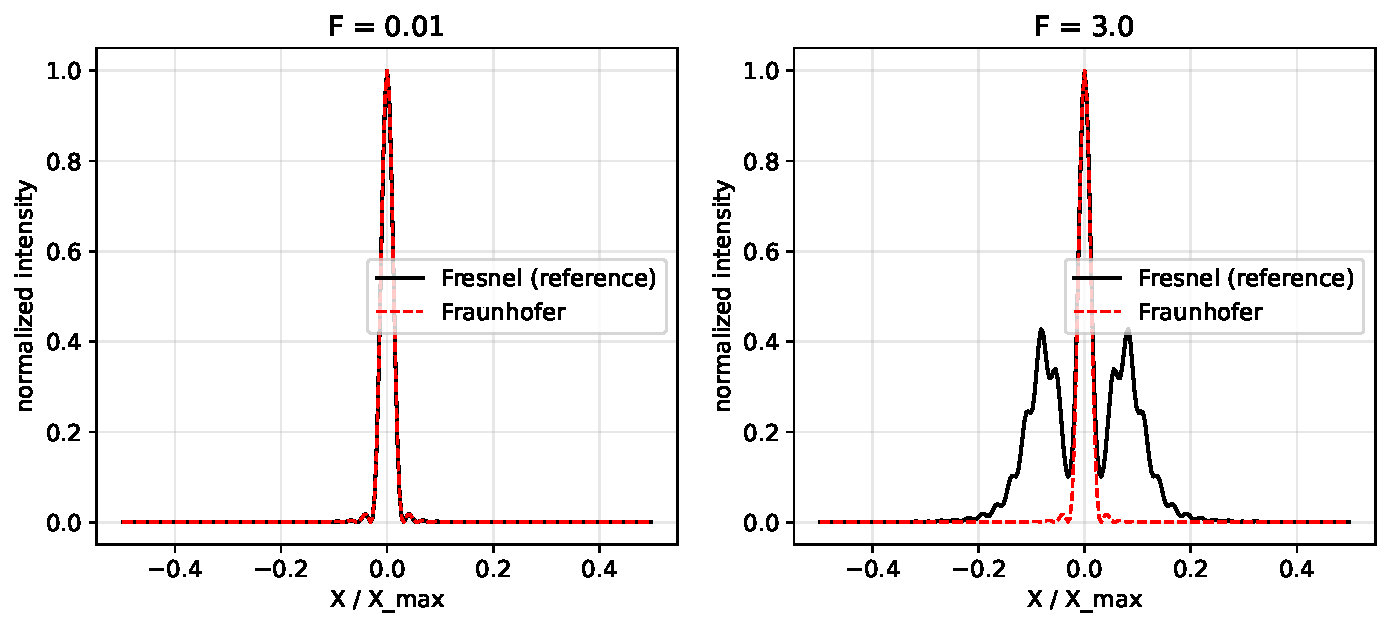
\includegraphics[width=0.49\textwidth,height=0.58\textheight,keepaspectratio]{experiment4_patterns.pdf}
    \end{center}

    \vspace{-0.10cm}
    \small
    E3 is isolated by comparing Fraunhofer with the Fresnel/ASM reference. For small \(F\), the fitted
    slope is \(2.00\); around \(F=1\), E3 is already about \(0.45\); for large \(F\), the Fraunhofer
    pattern is no longer reliable.
\end{frame}

\begin{frame}{Experiment 5: Efficiency}
    FFT and Simpson quadrature agree to roundoff on the Gaussian test, so runtime is the main difference.

    \vspace{0.25cm}
    \begin{center}
    \begin{tabular}{cccc}
        \toprule
        \(N\) & FFT time & Simpson time & Speedup \\
        \midrule
        64 & \(2.5\times10^{-4}\,\mathrm{s}\) & \(1.68\times10^{-1}\,\mathrm{s}\) & \(\sim670\times\) \\
        128 & \(9.6\times10^{-4}\,\mathrm{s}\) & \(2.09\,\mathrm{s}\) & \(\sim2200\times\) \\
        256 & \(9.4\times10^{-3}\,\mathrm{s}\) & \(61.6\,\mathrm{s}\) & \(\sim6500\times\) \\
        \bottomrule
    \end{tabular}
    \end{center}

    \vspace{0.2cm}
    \begin{block}{Takeaway}
        The FFT gives the same numerical result in the tested regime, but its cost scales like
        \(O(N^2\log N)\) instead of \(O(N^4)\).
    \end{block}
\end{frame}

\begin{frame}{Experiment 6: Rayleigh Recovery}
    For a circular aperture, the first Airy dark ring should satisfy
    \[
        r_1\approx 1.21967\,\frac{\lambda z}{D}.
    \]
    The numerical constant is recovered from
    \[
        c_{\mathrm{num}}=\frac{r_1D}{\lambda z}.
    \]

    \vspace{0.2cm}
    The experiment locates \(r_1\) from the central intensity cut using a three-point parabolic refinement.
\end{frame}

\begin{frame}{Experiment 6: Numerical Result}
    \begin{columns}[T,onlytextwidth]
        \column{0.58\textwidth}
        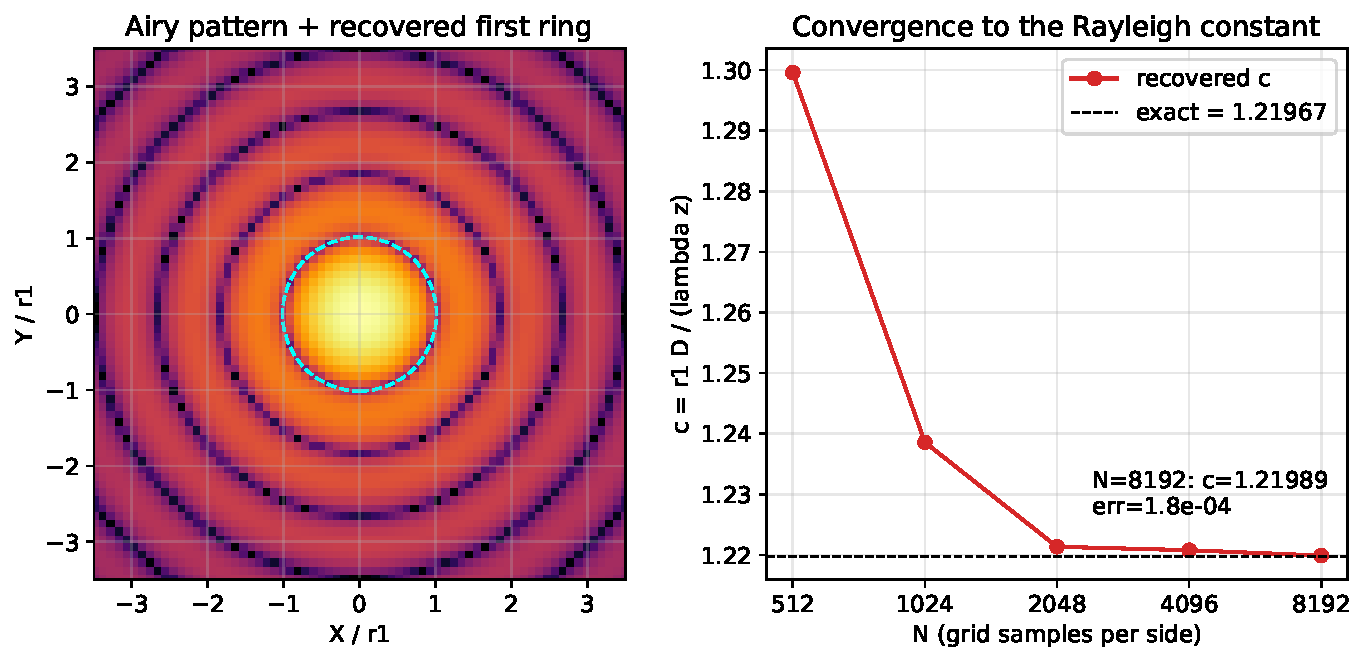
\includegraphics[width=\textwidth]{experiment6_rayleigh.pdf}

        \column{0.38\textwidth}
        \small
        \begin{center}
        \begin{tabular}{ccc}
            \toprule
            \(N\) & \(c_{\mathrm{num}}\) & rel. error \\
            \midrule
            512 & 1.299592 & \(6.55\%\) \\
            1024 & 1.238582 & \(1.55\%\) \\
            2048 & 1.221345 & \(0.137\%\) \\
            4096 & 1.220777 & \(0.0908\%\) \\
            8192 & 1.219887 & \(0.0178\%\) \\
            \bottomrule
        \end{tabular}
        \end{center}

        The value converges to \(1.21967\ldots\), confirming the Rayleigh scale \(1.22\lambda/D\).
    \end{columns}
\end{frame}

\begin{frame}{Experiment 7: Complex Apertures}
    \begin{columns}[T,onlytextwidth]
        \column{0.50\textwidth}
        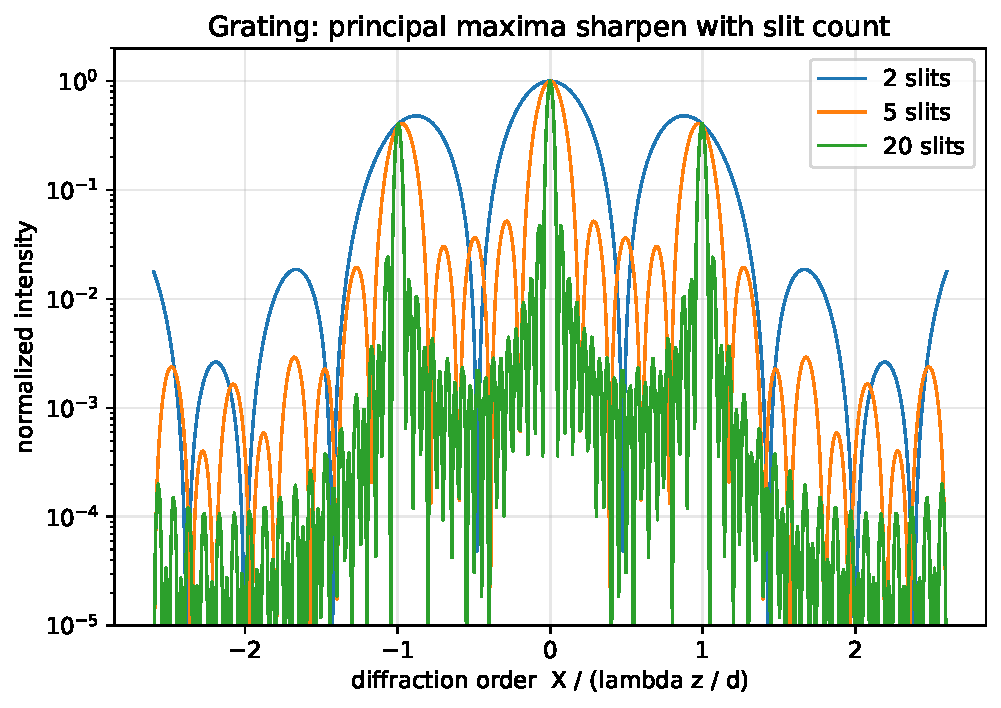
\includegraphics[width=\textwidth,height=0.30\textheight,keepaspectratio]{experiment7_grating_slitcount.pdf}

        \vspace{0.06cm}
        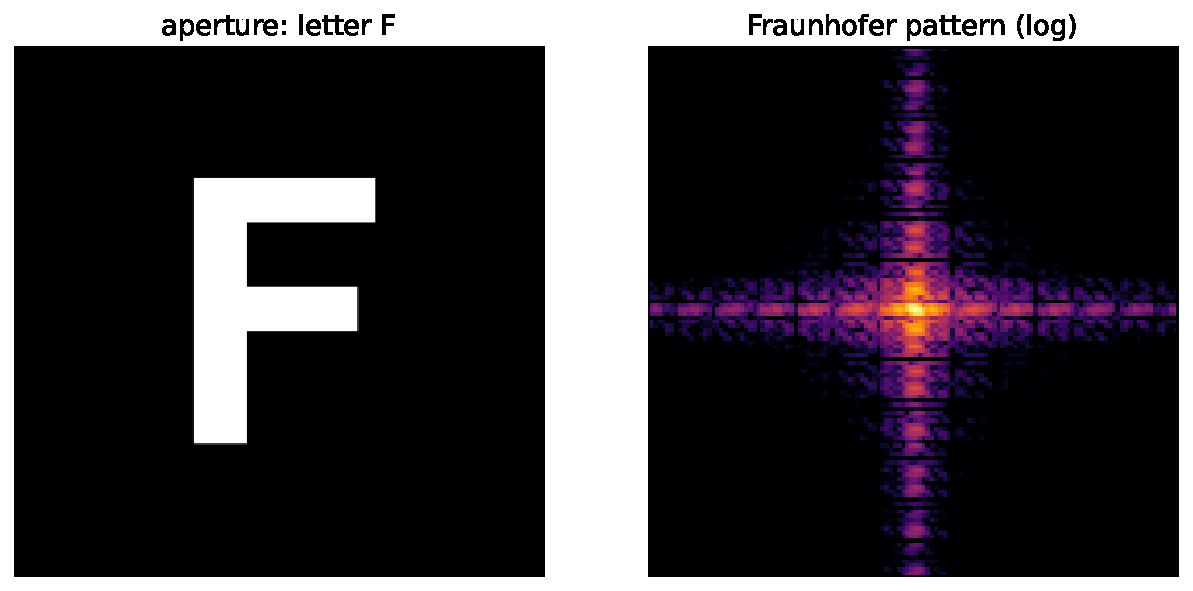
\includegraphics[width=\textwidth,height=0.30\textheight,keepaspectratio]{experiment7_letter.pdf}

        \column{0.50\textwidth}
        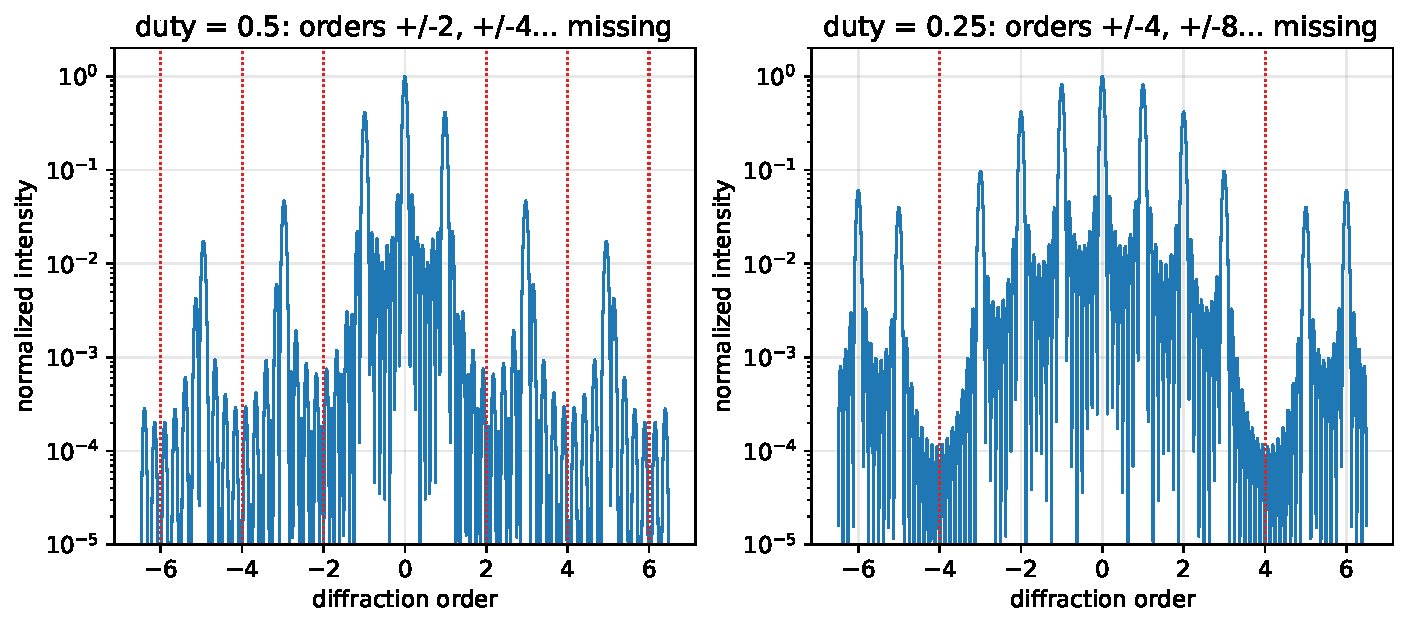
\includegraphics[width=\textwidth,height=0.30\textheight,keepaspectratio]{experiment7_grating_duty.pdf}

        \vspace{0.06cm}
        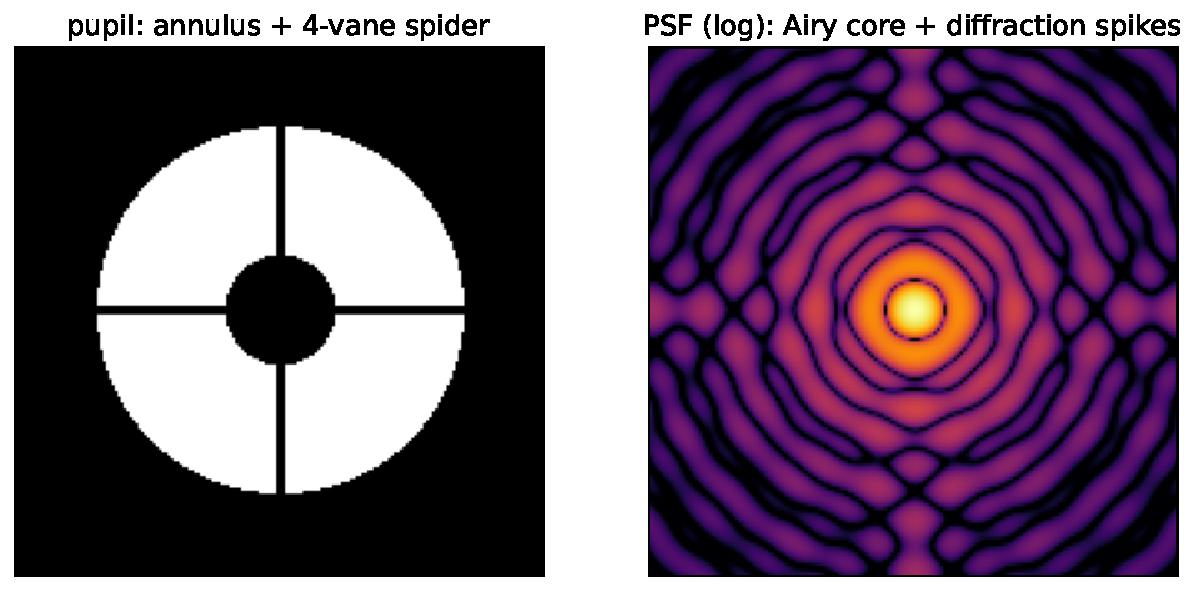
\includegraphics[width=\textwidth,height=0.30\textheight,keepaspectratio]{experiment7_telescope.pdf}
    \end{columns}

    \vspace{0.05cm}
    \small
    The same FFT pipeline handles gratings, letter-shaped apertures, and telescope pupils without changing
    the algorithm.
\end{frame}

\section{Conclusion}

\begin{frame}{Main Takeaways}
    \begin{enumerate}
        \item Fraunhofer diffraction reduces the far-field pattern to a Fourier transform of the aperture.
        \item The FFT is efficient, but its grid fixes both screen spacing and observable range.
        \item E1, E2, and E3 correspond to different mechanisms and must be controlled separately.
        \item Experiments confirm analytical patterns, convergence behavior, grid tightness, and model
              breakdown.
        \item The Rayleigh constant \(1.21967\ldots\) is numerically recovered from the Airy disk.
    \end{enumerate}
\end{frame}

\begin{frame}{References}
    \footnotesize
    \begin{thebibliography}{9}
        \bibitem{goodman2017}
        J. W. Goodman, \textit{Introduction to Fourier Optics}, 4th ed., W. H. Freeman, 2017.

        \bibitem{mit271}
        MIT OpenCourseWare, \textit{2.71 Optics}, Lectures 15--17.

        \bibitem{douglass}
        K. M. Douglass, ``Approximating Diffraction Patterns of Rectangular Apertures with the FFT,''
        \url{https://kmdouglass.github.io/posts/approximating-diffraction-patterns-of-rectangular-apertures-with-the-fft/}.
    \end{thebibliography}
\end{frame}

\begin{frame}
    \centering
    \Huge Thank you

    \vspace{0.5cm}
    \large Questions?
\end{frame}

\end{document}
